%%%%%%%%%%%%%%%%%%%%%%%%%%%%%%%%%%%%%%%%%%%%%%%%%%%%%%%%%%%%%%%%%%%%%%%%
%                                                                      %
%     File: Thesis_Conclusions.tex                                     %
%     Tex Master: Thesis.tex                                           %
%                                                                      %
%     Author: Andre C. Marta                                           %
%     Last modified :  2 Jul 2015                                      %
%                                                                      %
%%%%%%%%%%%%%%%%%%%%%%%%%%%%%%%%%%%%%%%%%%%%%%%%%%%%%%%%%%%%%%%%%%%%%%%%

\chapter{Analysis}
\label{chapter:analysis}

\section{Overview of the $hh\rightarrow b\overline{b}b\overline{b}$ channel}
- Signal cross section and final state signature \\
- Pros and challenges of using the 4b final state \\
- Main backgrounds (the ones we consider) and respective cross sections (leave for appendix discussion on other backgrounds, namely Higgs processes)\\
----------------------------------------------------------------\\

\begin{figure}
	\centering
	\includegraphics[width=0.6\textwidth]{./Figures/hhBR.png}
	\caption{Higgs pair branching ratios.}
\end{figure}

The searches for Higgs pair production in the four b quarks final state benefit from the large BR of $h\rightarrow b\overline{b}$. The value of this BR is $58\%$ making it the largest one among all Higgs boson decay modes. This leads to a cross section times BR of $\sim 0.7$ pb. However, in this channel, the main background is the QCD multijet production that has a very large cross section, of the order of $10^9$ pb. Nonetheless, it is a well known feature of QCD that the majority of jets produced are soft. This means that the $p_T$ distributions of this background have a very large yield close to zero and then fall very steeply while for the signal has a much larger tail to high values of $p_T$. This indicates that searches targeting the boosted kinematic regime may be the key to measure $hh\rightarrow b\overline{b}b\overline{b}$. In addition, the jets produced by QCD interaction are more likely to be initiated by a gluon or a light quark. Therefore, tight b-tagging criteria and sophisticated algorithms can also help reject this background. 

\subsection{Signal}

The experimental signature depends on the kinematic regime that is targeted. In the boosted regime, we expect at least two jets that are reconstructed using a large R parameter and that contain, each, the two b quarks that come from the decay of a Higgs boson. In the fully resolved regime, we expect at least four jets reconstructed with the standard R parameter of $0.4$, each corresponding to a b quark. Furthermore, an intermediate (or semi-resolved) category, in which one of the Higgs can be fully reconstructed using two small R jets and the other is reconstructed using a single large-R jet can also be explored. In all categories, we expect the presence of extra jets due to QCD activity. 

\subsection{Backgrounds}

In this work we include the QCD multijet background because of its huge cross section and the $t\overline{t}$ because the cross section is much larger than the signal, approximately $10^4$ pb, and the event topology is expected to be similar to the signal because it also consists in the production of a pair of particles with the same mass. The assumption that these are the two main backgrounds is corroborated by the ATLAS di-Higgs search performed in the same channel where these backgrounds are found to be the dominant ones and that all other sources of backgrounds, including processes involving Higgs bosons, are found to be negligible \cite{hh2bbbbATLAS}. In the appendix X we discuss and evaluate the importance of some backgrounds that include Higgs bosons to our analysis. In addition, we also take into account the irreducible background, $b\overline{b}b\overline{b}$.

\begin{figure}
\centering
\feynmandiagram
[horizontal=a to b] {i1 [particle=\(q\)] -- [fermion] a -- [fermion] i2 [particle=\(\overline{q}\)],a -- [gluon,edge label=\(g\)] b, f1 [particle=\(t\)] -- [fermion] b -- [fermion] f2 [particle=\(\overline{t}\)],
};\qquad
\feynmandiagram
[horizontal=a to b] {i1 [particle=\(g\)] -- [gluon] a -- [gluon] i2 [particle=\(g\)],a -- [gluon,edge label=\(g\)] b, f1 [particle=\(t\)] -- [fermion] b -- [fermion] f2 [particle=\(\overline{t}\)],
}; \qquad
\feynmandiagram[layered layout,horizontal=a to b] {% Draw the top and bottom lines
	i1 [particle=\(g\)]-- [gluon] a-- [anti fermion]  b [particle=\(\overline{t}\)] -- ,i2 [particle=\(g\)]-- [gluon] c-- [fermion] d [particle=\(t\)] -- ,
	% Draw the two internal fermion lines
	{ [  same layer] a -- [fermion] c},
};
\caption{Dominant diagrams of $pp\rightarrow t\overline{t}$ at LO.}
\end{figure}

\begin{figure}
	\centering
	\feynmandiagram[small,layered layout,horizontal=i1 to a] {% Draw the top and bottom lines
		i1 [particle=\(\overline{q}\)]-- [anti fermion] a-- [boson, edge label'=\(g/h/Z/\gamma\)]  b,
		i2 [particle=\(q\)]-- [fermion] c-- [gluon, edge label=\(g\)] d,
		% Draw the two internal fermion lines
		{ [  same layer] a -- [anti fermion] c},
		%f1  -- [fermion] b -- [fermion] f2 ,
		%f3  -- [fermion] f2 -- [gluon] g1 ,
		%f4  -- [fermion] g1 -- [fermion] f5 ,
	%	a -- [opacity=0.2] c,
		%g1 -- [anti fermion] b,
		b -- [anti fermion] f2 [particle=\(\overline{b}\)],
		b -- [fermion] f3 ,
		f3 -- [fermion] f4 [particle=\(b\)],
		f3 -- [boson, edge label'=\(g/h/Z/\gamma\)] g1,
		g1 -- [anti fermion] f5 [particle=\(\overline{b}\)],
		g1 -- [fermion] f6 [particle=\(b\)],
	};\qquad
		\feynmandiagram[small,layered layout,horizontal=a to b] {% Draw the top and bottom lines
			i1 [particle=\(\overline{q}\)]-- [anti fermion] a-- [anti fermion]  b,
			i2 [particle=\(q\)]-- [fermion] c-- [fermion] d [particle=\(q\)],
			% Draw the two internal fermion lines
			{ [  same layer] a -- [gluon] c},
			%f1  -- [fermion] b -- [fermion] f2 ,
			%f3  -- [fermion] f2 -- [gluon] g1 ,
			%f4  -- [fermion] g1 -- [fermion] f5 ,
			%	a -- [opacity=0.2] c,
			%g1 -- [anti fermion] b,
			b -- [anti fermion] f2 [particle=\(\overline{q}\)],
			b -- [gluon] f3 [particle=\(g\)],
		};\qquad
		\feynmandiagram
		[horizontal=a to b] {i1 [particle=\(q\)] -- [fermion] a -- [fermion] i2 [particle=\(\overline{q}\)],
			a -- [gluon] b,
			g1 -- [gluon] b -- [gluon] g2,
			f1 [particle=\(\overline{q}\)] -- [fermion] g1 -- [fermion] f2 [particle=\(q\)],
			f3 [particle=\(\overline{q}\)] -- [fermion] g2 -- [fermion] f4 [particle=\(q\)],
			g1 -- [opacity=0] g2,
			f2 -- [opacity=0] f4,
		};
%		\feynmandiagram[small,layered layout,horizontal=i1 to a] {% Draw the top and bottom lines
%			i1 [particle=\(\overline{q}\)]-- [anti fermion] a-- [boson, edge label'=\(h/Z/\gamma\)]  b,
%			i2 [particle=\(q\)]-- [fermion] c-- [gluon, edge label=\(g\)] d,
%			% Draw the two internal fermion lines
%			{ [  same layer] a -- [anti fermion] c},
%			%f1  -- [fermion] b -- [fermion] f2 ,
%			%f3  -- [fermion] f2 -- [gluon] g1 ,
%			%f4  -- [fermion] g1 -- [fermion] f5 ,
%			%	a -- [opacity=0.2] c,
%			%g1 -- [anti fermion] b,
%			b -- [anti fermion] f2 [particle=\(\overline{b}\)],
%			b -- [fermion] f3 ,
%			f3 -- [fermion] f4 [particle=\(b\)],
%			f3 -- [boson, edge label'=\(h/Z/\gamma\)] g1,
%			g1 -- [anti fermion] f5 [particle=\(\overline{b}\)],
%			g1 -- [fermion] f6 [particle=\(b\)],
%		};
	\caption{Example of diagrams that contribute to the QCD multijet background: five final state jets, four of which are b-jets (left), three final state jets (middle) and four final state jets (right). Here, $q$ stands for a light quark/jet.}
\end{figure}
%\begin{figure}[h]
%	\centering
%	\feynmandiagram [horizontal=b to c] {
%		a -- [gluon] b [blob],c -- [scalar] b-- [gluon] d,
%		c -- [scalar] e,
%		c -- [scalar] f,
%		e -- [fermion] g,
%		e -- [anti fermion] h,
%		f -- [fermion] i,
%		f -- [anti fermion] j,
%	};
%	\caption{Final state}
%\end{figure}

%\begin{figure}[h]
%	\centering
%	\feynmandiagram [horizontal=d to h] {
%		a [particle=\(g\)] -- [gluon] b [blob],
%		c [particle=\(g\)] -- [gluon] b -- [gluon],
%		d -- [scalar, edge label'=\(h\)] b -- [scalar],
%		e -- [scalar, edge label'=\(h\)] b -- [scalar],
%		d -- [fermion, edge label=\(b\)] g ,
%		d -- [anti fermion, edge label=\(\overline{b}\)] h ,
%		e -- [fermion, edge label'=\(b\)] i,
%		e -- [anti fermion, edge label'=\(\overline{b}\)] j ,
%		d -- [opacity=0] e,
%		%h -- [opacity=0] i,
%		g -- [opacity=0] h,
%		i -- [opacity=0] j,
%		h -- [opacity=0] i,
%	};
%	\caption{Final state}
%\end{figure}




%\begin{table}
%	\centering
%	\begin{tabular}{lp{30mm}p{10mm}p{30mm}p{30mm}}
%		\toprule 
%		Pythia & hh (h$\rightarrow b\overline{b}$) & 4b+j & jj+0/1/2 j & tt+0/1/2 j \\
%		\midrule
%		Relevant settings & 25:onMode=off \newline 25:onIfAny= 5 -5&  & \textbf{Jet matching:} \newline merge=on \newline scheme=1 \newline setMad=off \newline coneRadius=1.0 \newline etaJetMax=10 \newline nJetMax=4 \newline qCut=30 & \textbf{Jet matching:} \newline merge=on \newline scheme=1 \newline setMad=off \newline coneRadius=1.0 \newline etaJetMax=10 \newline nJetMax=2 \newline qCut=60\\
%		\rowcolor{black!7} Description & Turn on the $h\rightarrow b\overline{b}$ decay for the undecayed Higgs. &  &  \multicolumn{2}{l}{Set parameters for jet matching procedure. } \\
%		\bottomrule
%	\end{tabular}
%	\caption{oi}
%	\label{table:DelphesHCAL}
%\end{table}

\section{Analysis strategy}
\label{section:regions}

-------------------------------------------------------------------\\
%In this analysis we explore three regions: boosted, intermediate and resolved. The details about each region, namely the event topology and selection cuts, are discuss in the following sections (\ref{section:boosted}, \ref{section:intermediate} and \ref{section:resolved}). The regions are orthogonal, i.e, independent. For each event we check if it falls in the boosted category. If it does not we check if it falls in the intermediate category and if it does not we check if it falls in the resolved category. This way, an event falling in the boosted category cannot fall in the intermediate or resolved categories and the same applies for all categories. 
%
%The advantage of performing an analysis in orthogonal regions is that we can then combine the results obtained in each one. For example, we can quadratically add the significances in order to obtained an overall significance. This would not be possible if there were any overlap between the regions. In addition, we have access to increased statistics because we are exploring three different signal topologies. Nonetheless, the selection criteria for each category, as well as the variables to explore, are different and need to be optimized independently.

- Event topology: two boosted jets each corresponding to a Higgs \\
- Physics objects: partile flow anti-kT R=0.8 jets (discussion about jet radius in appendix) \\
- Selection criteria\\
- Substructure variables \\
- Optimization (efficiency plots, correlations, MVA...)\\
-------------------------------------------------------------------

\begin{figure}
	\centering
	\includegraphics[width=\textwidth]{./Figures/boosted1.png}
	%\hfill
	%\includegraphics[width=.45\textwidth]{./Figures/inter.png}
	\caption{Event topology targeted by the boosted analysis region. The blob represents the interaction between the gluons and the Higg bosons that is represented by the Feynman diagrams shown in figure \ref{fig:higgs_pair}.}
	\label{fig:final_state}
\end{figure} 

This analysis category targets events in which the Higgs bosons have a high Lorentz boost which leads to the collimation of the pairs of b quarks resulting from their decay. As a result, the b quarks cannot be reconstructed in four separated jets. Therefore, two pairs of b quarks are reconstructed using two jets with a larger R parameter. Each jet contains the b quarks coming from one of the Higgs bosons and works as a proxy for the properties of that Higgs boson.

The events are reconstructed using particle flow jets with $R=0.8$\footnote{Find discussion about jet radius in the appendix.}, clustered with the anti-$k_T$ algorithm. We perform the b-tagging of jets using truth level information as it is described in the following section \footnote{Jets with a large R parameter cannot be b tagged using Delphes default algorithm because the tagging of large R jets is an ambiguous task that can be performed in several different ways. Therefore, we need to implement our own b tagging algorithm/strategy.}. 

\subsection{Implementation of b-tagging}

For each jet, the two hardest subjets are found using the mass drop procedure. It might happen that there are not two subjets because the algorithm's criteria are not met. In that case, the jet is rejected. We compute the $\Delta R$ distance between all b and c quarks in the event with Pythia 8 status equal to $23$ \footnote{These are the partons that come from the hardest subprocess.} and with $p_T>10$ GeV and each subjet, $\Delta R(\text{subjet,parton})$. We consider that a subjet is matched to a given quark if $\Delta R(\text{subjet,parton})<0.3$. If the subjet is matched to at least a b quark, we b-tag the subjet with a given probability. If the subjet is not matched to any b quark but it is matched to at least one c quark we apply a c mistag rate. If the subjet is not matched to any b or c quark we apply a light mistag rate. The b-tag probability and mistag rates were obtained from the Delphes FCC-hh card. They depend on the momentum of the jet and on its $\eta$ coordinate. They are summarized in Table \ref{table:btag}. Note that a jet cannot be b-tagged if $|\eta|>4$ or if its momentum is smaller than $10$ GeV or larger than $15000$ GeV.  

\begin{table}
	\centering
	\begin{tabular}{llll}
		\toprule 
		\backslashbox{$\eta$}{$p_T$} & $10<p_T<500$ & $500<p_T<15000$ &  \\
		\midrule
		$|\eta|<2.5$ & $0.85;\textcolor{blue}{0.05};\textcolor{red}{0.01} $ & $(0.85;\textcolor{blue}{0.05};\textcolor{red}{0.01})\times\left(1-p_T/15000\right)$ &   \\
		\rowcolor{black!7} $2.5<|\eta|<4.0$ & $0.64;\textcolor{blue}{0.03};\textcolor{red}{0.0075}$ & $(0.64;\textcolor{blue}{0.03};\textcolor{red}{0.0075})\times\left(1-p_T/15000\right)$ &  \\
		\bottomrule
	\end{tabular}
	\caption{b-Tagging (black), c (blue) and light (red) mistag probabilities as a function of $\eta$ and $p_T$ of the (sub)jet. The momentum dependent factor, $\left(1-p_T/15000\right)$, is common to the three probabilities.}
	\label{table:btag}
\end{table}

[PLOT OF DELTA R (b,subjet)]


\subsection{Event selection}

We require at least two b-tagged jets with $|\eta|<6$. We require that the leading and sub leading jets have $p_T>200$ GeV. 

\subsection{Optimization}

%% ----------------------------------------------------------------------
%\subsection{Intermediate}
%\label{section:intermediate}
%
%- Event topology: one large R jet corresponding to the leading Higgs candidate and two small R jets corresponding to the b quarks of the sub leading Higgs candidate \\
%- Physics objects: fat jets (already described in previous section) and particle flow anti-kT R=0.4 jets \\
%- Selection criteria \\
%- Substructure variables: refer we (can)apply them to the fat jet \\
%- Optimization\\
%-------------------------------------------------------------------
% 
%This category targets events in which one of the Higgs bosons has a high Lorentz boost and therefore is reconstructed using a particle flow, anti-$k_T$ jet with $R=0.8$ (large-R jets). This is assumed to be the leading Higgs candidate. The sub leading Higgs boson, due to its relatively low $p_T$, can be fully reconstructed, meaning that each b quark is reconstructed using particle flow, anti-$k_T$ jets with $R=0.4$ (small-R jets). For the large-R jets the b-tagging is performed as described in the previous section. The small-R jets are b-tagged using Delphes default algorithm.
%
%\subsubsection{Event selection}
%
%We require exactly one large-R jet and at least two small-R jets. All jets have to be within $|\eta|<6$. The large-R jet is required to have $p_T>200$ GeV and the small-R jets are required to have $p_T>50$ GeV.
%% ----------------------------------------------------------------------
%\subsection{Resolved}
%\label{section:resolved}
%
%- Event topology: 4 small-R jets \\
%- Physics objects: small R jets already described in previous section \\
%- Selection criteria \\
%- Optimization (angular variables between b quarks, ...)\\
%-------------------------------------------------------------------
%
%This analysis category targets events in which the four b quarks can be reconstructed in four individual jets.
%
%The events are reconstructed using particle flow jets with $R=0.4$, clustered with the anti-$k_T$ algorithm. The b tagging is done using Delphes default algorithm.